%!TEX encoding = UTF-8 Unicode
\documentclass{beamer}
\usepackage{amsmath,amsthm,amssymb}
\usepackage{CJKutf8}
\usepackage{graphicx}
\usepackage{hyperref}
\usepackage{pstricks-add}

\hypersetup{colorlinks,linkcolor=,unicode}
\useoutertheme{sidebar}
\usecolortheme{rose}
\usecolortheme{seahorse}
\newcommand{\Left} {\mathopen{}\mathclose\bgroup\left}
\newcommand{\Right}{\aftergroup\egroup\right}
\newcommand  {\e}{\text e}
\renewcommand{\i}{\text i}
\newcommand  {\N}{\mathbb N}
\newcommand  {\Z}{\mathbb Z}
\newcommand  {\Q}{\mathbb Q}
\newcommand  {\R}{\mathbb R}
\renewcommand{\C}{\mathbb C}
\newcommand{\sech}  {\operatorname{sech}}
\newcommand{\csch}  {\operatorname{csch}}
\newcommand{\arsinh}{\operatorname{arsinh}}
\newcommand{\op}  {\operatorname{op}}
\newcommand{\Elem}{\operatorname{Elem}}
\newcommand{\trig}{\operatorname{trig}}
\renewcommand{\today}{\number\year~年~\number\month~月~\number\day~日}
\newcommand{\negskip}{\vskip -2em plus 3pt minus 3pt}

\theoremstyle{remark}
  \newtheorem{remark}{Remark}

\title{積分}
\author[何震邦]{何震邦 \href{mailto:jdh8@ms63.hinet.net}{\textless jdh8@ms63.hinet.net\textgreater}\\
    \href{http://creativecommons.org/licenses/by-sa/3.0/tw/deed.zh\textunderscore TW}{\includegraphics{by-sa.eps}}}

\begin{document}
\begin{CJK}{UTF8}{bsmi}
\maketitle

\section{積分}
\begin{frame}{積分的用途}
  \begin{columns}
    \begin{column}{0.5\textwidth}
      \begin{itemize}
	\item 求面積與體積
	  \begin{itemize}
	    \item 求轉動慣量
	  \end{itemize}
	\item 解微分方程
	  \begin{itemize}
	    \item 變力作功
	    \item 訊號處理
	  \end{itemize}
      \end{itemize}
    \end{column}
    \begin{column}{0.5\textwidth}
      \begin{center}
	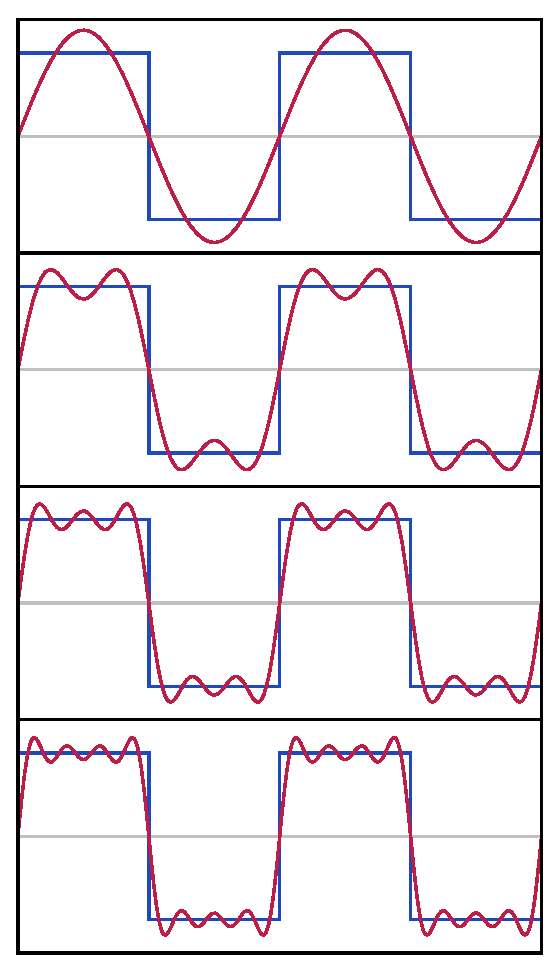
\includegraphics[height=0.8\textheight]{FourierSeries}
      \end{center}
    \end{column}
  \end{columns}
\end{frame}

\subsection{積分}
\begin{frame}{區間的分割}
  閉區間 $[a,b]$ 的一個\textbf{分割}是指在此區間中取有限的序列 $x_i$ 使得 $a = x_0 < x_1 < \cdots < x_n = b$。每個閉區間
  $[x_i, x_{i+1}]$ 叫做一個\textbf{子區間}。
\end{frame}

\begin{frame}{黎曼--達布和}
  設 $f: [a,b] \to \R$ 是有界函數,且 $P: x_0, \dots, x_n$ 是閉區間 $[a,b]$ 的一個分割。設
  \begin{align*}
    M_i &= \sup_{x \in [x_i, x_{i+1}]} f(x)\\
    m_i &= \inf_{x \in [x_i, x_{i+1}]} f(x).
  \end{align*}
  $f$ 在分割 $P$ 下的\textbf{上黎曼和}為
  \[\sum_{i=0}^{n-1} M_i \left( x_{i+1} - x_i \right)\]
  而\textbf{下黎曼和}為
  \[\sum_{i=0}^{n-1} m_i \left( x_{i+1} - x_i \right).\]
\end{frame}

\begin{frame}{黎曼--達布積分}
  \begin{columns}
    \begin{column}{0.5\textwidth}
      $f$ 的\textbf{上達布積分}是所有上黎曼和的下確界,而 $f$ 的\textbf{下達布積分}是所有下黎曼和的上確界。

      若 $f$ 的上下達布積分相等,則我們說 $f$ 是黎曼--達布可積,且定義此積分為
      \[\int_a^b f(x)\,dx.\]
    \end{column}
    \begin{column}{0.5\textwidth}
      \begin{center}
	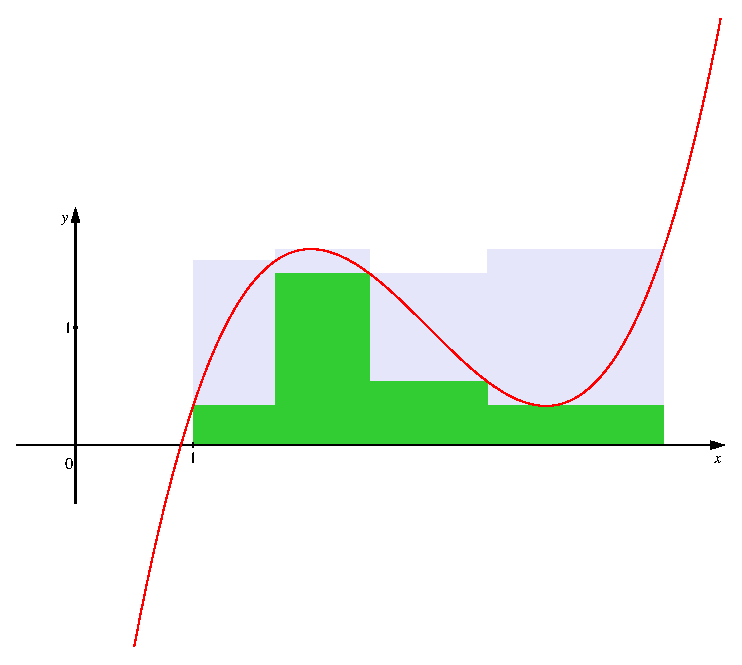
\includegraphics[width=\textwidth]{Darboux}
      \end{center}
    \end{column}
  \end{columns}
\end{frame}

\subsection{微積分基本定理}
\begin{frame}{微積分基本定理,第一部份}
  設 $f$ 是在閉區間 $[a,b]$ 中連續的實函數。設 $F$ 在區間 $[a,b]$ 中定義為
  \[F(x) = \int_a^x f(t)\,dt\]
  則 $F$ 在 $[a,b]$ 連續,在開區間 $(a,b)$ 可導,且 $\forall x \in (a,b)$
  \[F'(x) = f(x).\]
\end{frame}

\begin{frame}{微積分基本定理,第二部份}
  設 $f$ 和 $F$ 在閉區間 $[a,b]$ 上有定義,且 $F$ 的導函數為 $f$,即 $\forall x \in [a,b]$
  \[F'(x) = f(x).\]
  若 $f$ 在 $[a,b]$ 黎曼可積則
  \[\int_a^b f(x)\,dx = F(b) - F(a).\]
\end{frame}

\section{積分的技巧}
\begin{frame}{符號積分的困難}
  \begin{itemize}
    \item 初等函數的導函數仍是初等函數。
    \item 初等函數的反導函數就\textbf{不一定}是初等函數。
  \end{itemize}
\end{frame}

\begin{frame}{換元積分法}
  \[\int_{g(a)}^{g(b)} f(x)\,dx = \int_a^b f(g(t))\,g'(t)\,dt.\]
  \begin{proof}
    設函數 $F$ 使得 $F'(x) = f(x)$。
    \[(F \circ g)'(t) = F'(g(t))\,g'(t) = f(g(t))\,g'(t).\]
    \begin{align*}
      \int_a^b f(g(t))\,g'(t)\,dt &= F(g(b)) - F(g(a))\\
	&= \int_{g(a)}^{g(b)} f(x)\,dx. \qedhere
    \end{align*}
  \end{proof}
\end{frame}

\begin{frame}{分部積分法}
  \begin{align*}
    \int u(x)\,v'(x)\,dx &= u(x)\,v(x) - \int u'(x)\,v(x)\,dx\\
    \int u\,dv &= uv - \int v\,du.
  \end{align*}
  \begin{proof}
    \negskip
    \begin{align*}
      (u(x)\,v(x))' &= u'(x)\,v(x) + u(x)\,v'(x)\\
      \int_a^b (u(x)\,v(x))' dx &= \int_a^b u'(x)\,v(x)\,dx + \int_a^b  u(x)\,v'(x)\,dx\\
       \int_a^b  u(x)\,v'(x)\,dx &= \left[ u(x)\,v(x) \right]_a^b - \int_a^b u'(x)\,v(x)\,dx. \qedhere
    \end{align*}
  \end{proof}
\end{frame}

\subsection[乘冪、指對數的積分]{乘冪、指數與對數的積分}
\begin{frame}{冪函數與指數函數的積分}
  \begin{align*}
    \int x^a dx &= \frac{x^{a+1}}{a+1} & a \ne -1\\
    \int \frac{1}{x}\,dx &= \ln \Left| x \Right|\\
    \int b^x dx &= \frac{b^x}{\ln(b)}.\\
  \end{align*}
\end{frame}

\begin{frame}{$\displaystyle \int \ln \Left| x \Right|\,dx = x \ln \Left| x \Right| - x$}
  \begin{proof}
    設 $u = \ln \Left| x \Right|$,則 $du = \dfrac{1}{x}\,dx$。
    \begin{align*}
      \int \ln \Left| x \Right|\,dx &= \int u\,dx\\
	&= xu - \int x\,du\\
	&= x \ln \Left| x \Right| - \int dx\\
	&= x \ln \Left| x \Right| - x. \qedhere
    \end{align*}
  \end{proof}
\end{frame}

\subsection{三角函數的積分}
\begin{frame}{三角函數的積分}
  \begin{align*}
    \int \sin(x)\,dx &= -\cos(x)\\
    \int \cos(x)\,dx &= \sin(x)\\
    \int \tan(x)\,dx &= \ln \Left| \sec(x) \Right|\\
    \int \cot(x)\,dx &= \ln \Left| \sin(x) \Right|\\
    \int \sec(x)\,dx &= \ln \Left| \tan(x) + \sec(x) \Right|\\
    \int \csc(x)\,dx &= -\ln \Left| \csc(x) + \cot(x) \Right|.
  \end{align*}
\end{frame}

\begin{frame}{$\displaystyle \int \tan(x)\,dx = \ln \Left| \sec(x) \Right|$}
  \begin{proof}
    設 $u = \cos(x)$。
    \begin{align*}
      \int \tan(x)\,dx &= \int \frac{\sin(x)}{\cos(x)}\,dx\\
        &= \int -\frac{1}{u}\,du\\
	&= -\ln \Left| u \Right|\\
	&= \ln \Left| \sec(x) \Right|. \qedhere
    \end{align*}
  \end{proof}
\end{frame}

\begin{frame}{$\displaystyle \int \cot(x)\,dx = \ln \Left| \sin(x) \Right|$}
  \begin{proof}
    設 $u = \sin(x)$。
    \begin{align*}
      \int \cot(x)\,dx &= \int \frac{\cos(x)}{\sin(x)}\,dx\\
        &= \int \frac{1}{u}\,du\\
	&= \ln \Left| u \Right|\\
	&= \ln \Left| \sin(x) \Right|. \qedhere
    \end{align*}
  \end{proof}
\end{frame}

\begin{frame}{$\displaystyle \int \sec(x)\,dx = \ln \Left| \tan(x) + \sec(x) \Right|$}
  \begin{proof}
    設 $u = \tan(x) + \sec(x)$。
    \begin{align*}
      \int \sec(x)\,dx &= \int \frac{u \sec(x)}{u}\,dx\\
	&= \int \frac{\sec(x) \tan(x) + \sec(x)^2}{\tan(x) + \sec(x)}\,dx\\
        &= \int \frac{1}{u}\,du\\
	&= \ln \Left| u \Right|\\
	&= \ln \Left| \tan(x) + \sec(x) \Right|. \qedhere
    \end{align*}
  \end{proof}
\end{frame}

\begin{frame}{$\displaystyle \int \csc(x)\,dx = -\ln \Left| \csc(x) + \cot(x) \Right|$}
  \begin{proof}
    設 $u = \csc(x) + \cot(x)$。
    \begin{align*}
      \int \csc(x)\,dx &= \int \frac{u \csc(x)}{u}\,dx\\
	&= \int \frac{\csc(x)^2 + \csc(x) \cot(x)}{\csc(x) + \cot(x)}\,dx\\
        &= \int -\frac{1}{u}\,du\\
	&= -\ln \Left| u \Right|\\
	&= -\ln \Left| \csc(x) + \cot(x) \Right|. \qedhere
    \end{align*}
  \end{proof}
\end{frame}

\subsection{雙曲函數的積分}
\begin{frame}{雙曲函數的定義}
  \begin{align*}
    \cosh(x) &\triangleq \frac{\e^x + \e^{-x}}{2}\\
    \sinh(x) &\triangleq \frac{\e^x - \e^{-x}}{2}\\
    \tanh(x) &\triangleq \frac{\sinh(x)}{\cosh(x)}\\
    \coth(x) &\triangleq \frac{\cosh(x)}{\sinh(x)}\\
    \sech(x) &\triangleq \frac{1}{\cosh(x)}\\
    \csch(x) &\triangleq \frac{1}{\sinh(x)}.
  \end{align*}
\end{frame}

\begin{frame}{雙曲函數的性質}
  將三角函數的公式以 cos 和 sin 展開,若欲轉換為 cosh 和 sinh,則需每逢 2 個 sin 相乘\textbf{變號}。
  \[\cosh(x)^2 - \sinh(x)^2 = 1.\]
  \[\sinh(2x) = 2 \cosh(x) \sinh(x).\]
  原因:
  \[\sin(x) = \frac{\e^{\i x} - \e^{-\i x}}{2\i}.\]
\end{frame}

\begin{frame}{雙曲函數的導函數}
  \begin{align*}
    \frac{d}{dx} \sinh(x) &= \cosh(x)\\
    \frac{d}{dx} \cosh(x) &= \sinh(x)\\
    \frac{d}{dx} \tanh(x) &= \sech(x)^2\\
    \frac{d}{dx} \coth(x) &= -\csch(x)^2\\
    \frac{d}{dx} \sech(x) &= -\sech(x) \tanh(x)\\
    \frac{d}{dx} \csch(x) &= -\coth(x) \csch(x).
  \end{align*}
\end{frame}

\begin{frame}{$\displaystyle \frac{d}{dx} \arsinh(x)\,dx = \frac{1}{\sqrt{x^2 + 1}}$}
  \begin{proof}
    設 $y = \arsinh(x)$,則 $x = \sinh(y)$。
    \begin{align*}
      \frac{dx}{dy} &= \cosh(y)\\
      \frac{dy}{dx} &= \frac{1}{\cosh(y)} = \frac{1}{\sqrt{x^2 + 1}}. \qedhere
    \end{align*}
  \end{proof}
\end{frame}

\begin{frame}{雙曲函數的積分}
  \begin{align*}
    \int \sinh(x)\,dx &= \cosh(x)\\
    \int \cosh(x)\,dx &= \sinh(x)\\
    \int \tanh(x)\,dx &= \ln(\cosh(x))\\
    \int \coth(x)\,dx &= \ln \Left| \sinh(x) \Right|\\
    \int \sech(x)\,dx &= \arctan(\sinh(x))\\
    \int \csch(x)\,dx &= \ln \Left| \tanh \Left( \frac x 2 \Right) \Right|.
  \end{align*}
\end{frame}

\begin{frame}{$\displaystyle \int \sech(x)\,dx = \arctan(\sinh(x))$}
  \begin{proof}
    設 $u = \sinh(x)$。
    \begin{align*}
      \int \sech(x)\,dx &= \int \frac{\cosh(x)}{\sinh(x)^2 + 1}\,dx\\
	&= \int \frac{1}{u^2 + 1}\,du\\
	&= \arctan(u)\\
	&= \arctan(\sinh(x)). \qedhere
    \end{align*}
  \end{proof}
\end{frame}

\begin{frame}{$\displaystyle \int \csch(x)\,dx = \ln \Left| \tanh \Left( \frac x 2 \Right) \Right|$}
  \begin{proof}
    設 $u = \tanh \Left( \frac x 2 \Right)$。
    \begin{align*}
      \int \csch(x)\,dx &= \int \frac{1}{2 \cosh \Left( \frac x 2 \Right) \sinh \Left( \frac x 2 \Right)}\,dx\\
	&= \int \frac{\sech \Left( \frac x 2 \Right)^2}{2 \tanh \Left( \frac x 2 \Right)}\,dx\\
	&= \int \frac{1}{u}\,du\\
	&= \ln \Left| u \Right|\\
	&= \ln \Left| \tanh \Left( \frac x 2 \Right) \Right|. \qedhere
    \end{align*}
  \end{proof}
\end{frame}

\section{電腦代數系統}
\begin{frame}{\href{http://maxima.sourceforge.net/}{Maxima}------一套強大的電腦代數系統}
  \begin{itemize}
    \item 原始碼可在許多系統上編譯,包括 Windows、Linux、Mac OS X。
    \item 它的前身 Macsyma 是 1960 年代由 MIT 研發的。
      \begin{itemize}
	\item 感謝其自由開放的傳統,目前大型商業套件如 Maple 和 Mathematica 也是以它為藍本。
      \end{itemize}
    \item Maxima 是 \href{http://www.gnu.org/licenses/gpl-2.0.html}{GPL v2}
      下的自由軟體,我們可自由使用、研究、散布、改良。
      \begin{itemize}
	\item 我們可以站在巨人的肩膀上,不必重新發明輪子。
      \end{itemize}
  \end{itemize}
\end{frame}

\begin{frame}{\href{http://andrejv.github.com/wxmaxima/}{wxMaxima}------Maxima 的介面}
  多語言圖形介面,含中文,還有漂亮的輸出。
  \begin{center}
    \href{http://andrejv.github.com/wxmaxima/}{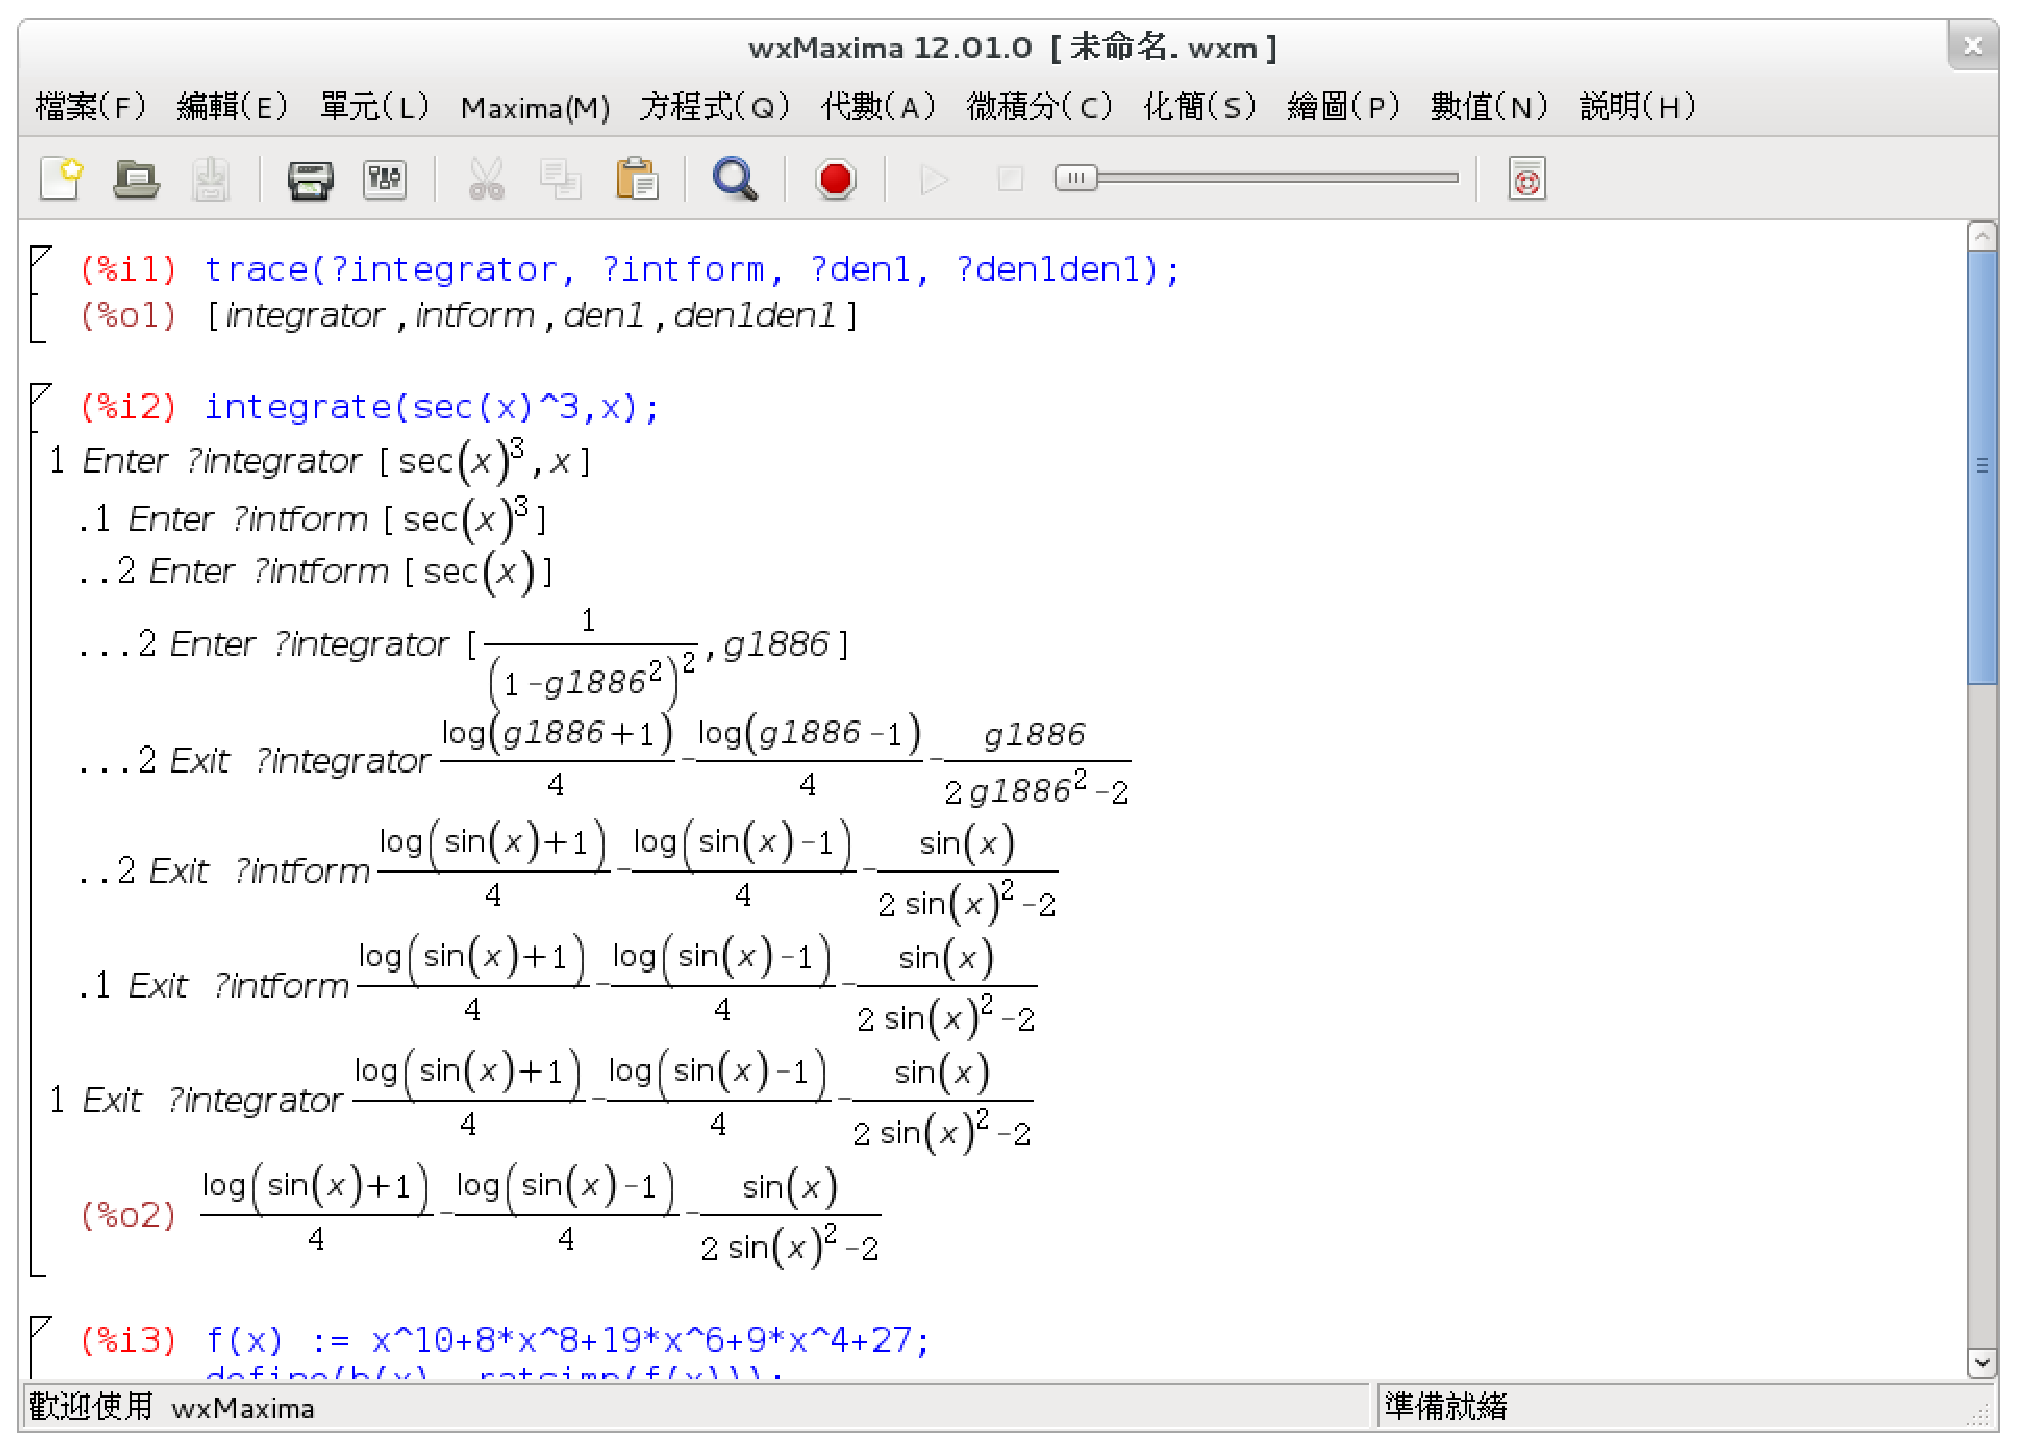
\includegraphics[width=0.8\textwidth]{screenshot}}
  \end{center}
\end{frame}

\begin{frame}
  \begin{center}
    \huge Tanks for your attention!
  \end{center}
\end{frame}
\end{CJK}
\end{document}
